\section{Results}

\newlength\figurewidth
\setlength\figurewidth{0.45\textwidth}

\begin{figure*}
  \centering
  \subcaptionbox{
    Bus Occupancy as a function of stop length.
    Occupancy is measured after each passenger transaction (e.g. a transaction taking 10s and adding 5 passengers to an existing pool of 20 would be charted as (10,25)).
    Stop length has no apparent correlation to Occupancy.
    \label{fig:occ}
  }[0.48\linewidth]{
    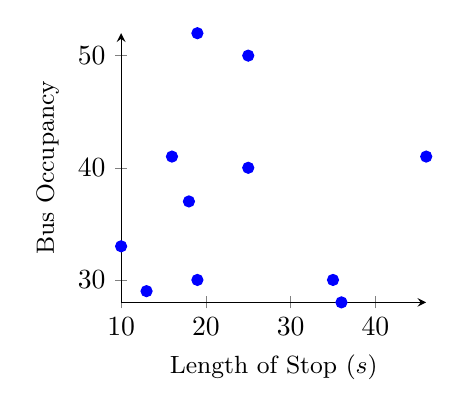
\begin{tikzpicture}
      \begin{axis}[
          axis x line=bottom,
          axis y line=left,
          width=\figurewidth,
          height=5cm,
          xlabel={\small Length of Stop ($s$)},
          ylabel={\small Bus Occupancy}]
        \addplot[only marks,mark=*,blue] plot coordinates {
          (35,30)  % BCC
          (18,37)  % Buell
          (16,41)  % Werblin
          (46,41)  % Scoot
          (25,50)  % SAC
          (19,52)  % Stadium
          %(9,52)  % Werblin 2
          (25,40)  % Hill
          (19,30)  % ARC
          (13,29)  % LSM
          (10,33)  % Suites
          (36,28)  % BCC
        };
      \end{axis}
    \end{tikzpicture}
  }
  \subcaptionbox{
    Net Delta Occupancy as a function of stop length.
    No immediate relationship visible, however negative occupancy changes seem to be exclusive to larger stop lengths.
    \label{fig:netdelta}
  }[0.48\linewidth]{
    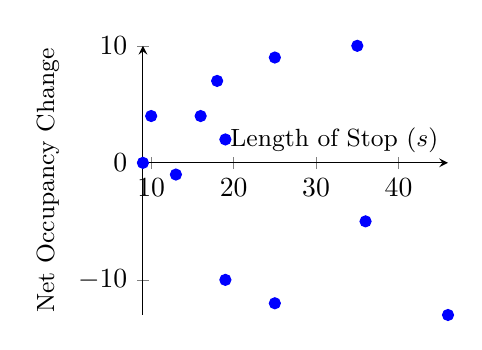
\begin{tikzpicture}
      \begin{axis}[
          axis x line=middle,
          axis y line=left,
          width=\figurewidth,
          height=5cm,
          xlabel={\small Length of Stop ($s$)},
          ylabel={\small Net Occupancy Change}]
        \addplot[only marks,mark=*,blue] plot coordinates {
          (35,10)  % BCC
          (18,7)  % Buell
          (16,4)  % Werblin
          (46,-13)  % Scoot
          (25,9)  % SAC
          (19,2)  % Stadium
          (9,0)  % Werblin 2
          (25,-12)  % Hill
          (19,-10)  % ARC
          (13,-1)  % LSM
          (10,4)  % Suites
          (36,-5)  % BCC
        };
      \end{axis}
    \end{tikzpicture}
    }
    \subcaptionbox{
      Absolute Delta Occupancy as a function of stop length.
      Strong correlation between magnitude of change and stop length.
      We can predict changes if we can show certain bus stops tend to positive or negative change.
      \label{fig:absdelta}
    }[0.48\linewidth]{
      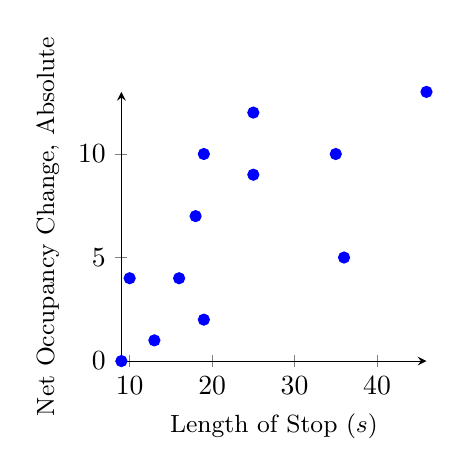
\begin{tikzpicture}
        \begin{axis}[
            axis x line=bottom,
            axis y line=left,
            width=\figurewidth,
            height=5cm,
            xlabel={\small Length of Stop ($s$)},
            ylabel={\small Net Occupancy Change{,} Absolute}]
          \addplot[only marks,mark=*,blue] plot coordinates {
            (35,10)  % BCC
            (18,7)  % Buell
            (16,4)  % Werblin
            (46,13)  % Scoot
            (25,9)  % SAC
            (19,2)  % Stadium
            (9,0)  % Werblin 2
            (25,12)  % Hill
            (19,10)  % ARC
            (13,1)  % LSM
            (10,4)  % Suites
            (36,5)  % BCC
          };
        \end{axis}
      \end{tikzpicture}
    }
    \subcaptionbox{
      Net Delta Occupancy as a function of Stop Length at a Single Stop.
      This supports the idea that we can characterize individual bus stops as being prone to positive or negative change.
      \label{fig:onestop}
    }[0.48\linewidth]{
      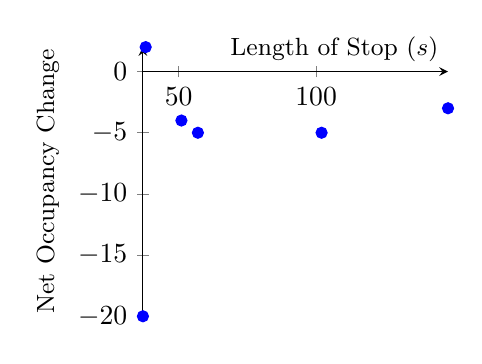
\begin{tikzpicture}
        \begin{axis}[
            axis x line=middle,
            axis y line=left,
            width=\figurewidth,
            height=5cm,
            xlabel={\small Length of Stop ($s$)},
            ylabel={\small Net Occupancy Change}]
          \addplot[only marks,mark=*,blue] plot coordinates {
            (37,-20)
            (51,-4)
            (38,2)
            (57,-5)
            (148,-3)
            (102,-5)
          };
        \end{axis}
      \end{tikzpicture}
    }
    \label{fig:busplots}
    \caption{
      Plots created with data from visual occupancy observation.
      Aside from \subref{fig:onestop}, which was created from the data from the $H$ route single-stop observation, these plots use the data from observation of the $A$ route.
    }
\end{figure*}


\subsection{Stop Length Inference}

Based on the experimental procedure described in TODO, Figure~\ref{fig:occ} depicts a lack of significant correlation between stop length and occupancy.
This makes sense, because the number of sedentary or otherwise intransient riders does not cause slowdowns; rather, the relevant metric is the net occupancy change; the number of people entering or exiting the bus at any given stop.
Plotting the net occupancy change as a function of stop length (Fig.~\ref{fig:netdelta}), however, was also inconclusive, as the longer stops could signify either positive or negative changes.
From stop timings alone, we would not be able to predict the direction of change.

Plotting absolute change (Fig.~\ref{fig:absdelta}), however, shows a much stronger correlation than either of the previous graphs.
Absolute change is not a useful metric on its own, but if it could be proven that certain bus stops tended to have a generally positive or negative net change, we could predict the sign of the change and thus the occupancy changes over time.
In other words, if more people tend to get on at a given stop than get off, a longer stop here means a large positive change to the number of passengers.
Conversely, a stop which is associated mostly with disembarking, a long stop would mean a large negative change.

To test this, we waited at a single bus stop and counted the number of passengers entering and leaving each bus on a certain route, and the length of the stops (Fig.~\ref{fig:onestop}).
Data for this experiment was slower to collect, as the buses were spaced out.
This data suggests that this particular bus stop is predominantly a destination, rather than a starting point; longer stops here, then, would imply a net decrease in number of riders.

However, the data collected was insufficient to draw these conclusions; there can be significant variation depending on time and day of the week.
This data collection would need to be repeated at every bus stop, on a variety of days and times, in order to provide the required basis of prediction.
This clearly increases the time requirement to well beyond the scope of this study.

Thus, while the preliminary foray suggests that this approach could be successful, it is not feasible for this study.
We move on to our next approach.

\subsection{Promiscuous WiFi}

\subsubsection*{Packet Plot}
\minifig{packets}{Packets detected per 3-second bin: there are visible differences between spots, and frequencies are higher on busier stops.}{fig:buspackets}

In figure~\ref{fig:buspackets}, we plot the number of packets in three second bins.
Analyzing this figure, we see that there are visible differences between stops.
This roughly lines up to the expected traffic around each stop --- stops like the BCC, Hill, the ARC, and the entirety of College Avenue have a large amount of traffic, while stops near the Visitor's Center and Werblin have very little.

\subsubsection*{Unique Devices Plot}
\minifig{unique}{Unique MAC addresses detected per 3-second bin: by plotting devices instead of packets, we get cleaner frequencies.}{fig:busunique}

Network traffic is not a good indicator of occupancy, however, because it represents the amount of activity, rather than the number of actors; a single person transmitting a large amount of data may be interpreted as multiple people with the Packet Plot.
As such, our next step was to switch out ``number of packets'' for ``number of unique MAC addresses'' (Fig.~\ref{fig:busunique}).
The Router filter would also be used here, since we don't want to count routers among the number of riders.
The values on this plot differ noticeably between stops.
However, this is not due to occupancy; there are clearly not nearly that many people on the bus.
Instead, it seems that the shape of the plot is primarily influenced by the proximity to routers --- the portions of the bus loop by athletic fields and between campuses has nearly no data.

\subsubsection*{First-Last Grid Plot}
\bigfig{bus-grid}{First and Last times seen for each MAC address observed while on the bus route: clumps along the line $y=x$ are noise. Points further from the line represent devices present for longer durations.}{fig:busgrid}
\bigfig{bus-hmap}{First and Last times seen for each MAC address observed while on the bus route: similar to previous plot, but clumps are easier to identify.}{fig:bushmap}

In order to establish which devices were on the bus, we plotted the time of the first and last occurrence of each device (Fig.~\ref{fig:busgrid}).
Each point here represents a unique device, where the x-coordinate is the time of the first sighting, and the y-coordinate is the time of the last sighting.
Thus, the high concentration of data points along the line \(y=x\) represents the transient devices, most likely people the bus was passing by.
The clump of data points in the top left corner of the plot represents devices which were seen throughout the journey.
These are most likely our own devices, or stationary devices around the geographically identical first and last stops.

As a variation on this, we also plotted the same data as a heat map (Fig.~\ref{fig:bushmap}), such that higher concentrations of points are depicted by more vivid colors.
In the original grid plot, any number of datapoints at the same coordinates would be shown the same as a single datapoint.
This method allows us to see more easily how many points are in each area of the plot (between Rutgers Student Center and SAC, for example).

\subsubsection*{Segments Plot}
\minifig{segments}{Predicted number of passengers using the Segments approximation (blue) versus actual number of passengers (purple). Segments approximation calculated from the intersection of sets of observed devices at each stop.}{fig:segments}
The segments plot was created using the procedure for segments plot described in the Graphing section.
The plot (Fig.~\ref{fig:segments}) shows the actual number of bus passengers as we observed (the purple function) overlayed with the function that we calculated using the lengths of each intersect-set (the blue function).
One can see that the calculated function is accurate for the stops after Werblin.
The discrepancy between the actual and calculated number of bus passengers at Buell (label 1) may be influenced by the fact that we had started observation and recording at this location. In this method, more routers equals more stop-to-stop change.
This fact means the calculated function will appear more accurate in areas with more devices.
There are more routers around the College Avenue areas, so the calculated function appears more accurate at these stops in comparison to stops like Werblin, which have fewer surrounding devices and routers.
Due to the limitations of this method, we progressed to creating the vector plot.

\subsubsection*{Presence Vector Plot}
\minifig{vectors}{Predicted number of passengers using the Vector approximation (blue) versus actual number of passengers (purple). Verctor approximation calculated by summing number of devices between first and last sightings.}{fig:vector}

In an attempt to minimize noise from transient devices and to compensate for the lack of traffic in uninhabited areas, we constructed a plot (Fig.~\ref{fig:vector}) similar to the previous.
For every address $i$ we encountered in the collection, we create a vector \(X^{(i)}= [ X_1 \cdots X_T ] \) such that
\begin{equation*}
  X_t^{(i)} = \begin{cases}
    1 & t_{\text{firstSeen}}^{(i)} \le t \le t_{\text{lastSeen}}^{(i)}\\
    0 & \text{otherwise}
  \end{cases}
\end{equation*}
with the sum of these vectors represented by $X$, such that \[X = \sum\limits_i X^{(i)}\]
The value at any point of $X$ indicates how many devices we can infer are presently on the bus.
Overlaid on this plot is the step function corresponding to the observed number of riders.
It is scaled differently, as there is approximately a three time difference between the devices seen and the people riding.

We see that there appears to be an excellent correlation here, with the exception of the 400-700 second segment. % uhh... what about 0-400? That's also pretty bad.
This segment corresponds to the entrance to the College Avenue campus, a highly concentrated area that appears to have contributed considerable noise.
We do see, however, that the two changes in occupancy in this region seem to correspond to peaks in the traffic --- this means that the traffic is probably higher than the actual by a constant value in that area, which we can account for in prediction. TODO: Roy's comment
